\documentclass[28pt,pdf,hyperref={unicode}]{beamer}
\usepackage[english,russian]{babel}

\usepackage[T2A]{fontenc}
\usepackage[utf8]{inputenc}
\usepackage{graphicx}
\usepackage{slashbox}
\usepackage{multirow}
\usepackage{xcolor,colortbl}
\usepackage{listings}

\usepackage{paratype}
\renewcommand*\familydefault{\sfdefault}

\usepackage{amsmath}
% \usepackage{inconsolata}
% \usepackage{fontspec}
% \setmonofont{Consolas}

\usepackage[customcolors]{hf-tikz}

\definecolor{mgreeen}{RGB}{27,158,119}
\definecolor{morange}{RGB}{217,95,2}
\definecolor{mblue}{RGB}{5,112,176}
\definecolor{mmagenta}{RGB}{231,41,138}

\definecolor{mtheme}{RGB}{130,130,130}
\definecolor{memph}{RGB}{50,50,50}

\definecolor{mgreen}{RGB}{0,109,44}
\definecolor{mred}{RGB}{203,24,29}



% \setbeamercolor{frametitle}{fg=black,bg=morange!50}
% \setbeamercolor{section in head/foot}{bg=morange}
% \setbeamercolor{author in head/foot}{bg=morange}
% % \setbeamercolor{date in head/foot}{fg=mblue}



\newcommand{\listing}[1]{\texttt{\colorbox{mlisting}{#1}}}
\newcommand{\foottt}[1]{\texttt{\footnotesize {#1}}}
\newcommand{\smalltt}[1]{\texttt{\small {#1}}}
\newcommand{\blue}[1]{\textcolor{blue}{#1}}

\renewcommand{\emph}[1]{\textbf{\color{memph}#1}}


\newcommand{\A}{\textbf{\textcolor{mmagenta}{A}}}
\renewcommand{\C}{\textbf{\textcolor{morange}{C}}}
\renewcommand{\G}{\textbf{\textcolor{mblue}{G}}}
\renewcommand{\U}{\textbf{\textcolor{mgreeen}{U}}}

\mode<presentation>
 {
\usetheme{Berlin}
\usecolortheme{seahorse}
 \setbeamercolor*{palette primary}{use=structure,fg=black,bg=mtheme!40}
 \setbeamercolor*{palette secondary}{use=structure,fg=black,bg=mtheme!40}
 \setbeamercolor*{palette tertiary}{use=structure,fg=black,bg=mtheme!40}
 \setbeamertemplate{itemize item}{\color{mtheme}\scriptsize$\blacksquare$}
\setbeamertemplate{itemize subitem}{\color{mtheme}\scriptsize$\blacktriangleright$}
 }

\parindent=0mm
% \parskip=.10in

\setbeamertemplate{headline}{}

\beamertemplatenavigationsymbolsempty

\setbeamertemplate{footline}
{
  \leavevmode
  \hbox{%
  \begin{beamercolorbox}[wd=.38\paperwidth,ht=2.25ex,dp=1ex,center]{author in head/foot}%
    \usebeamerfont{author in head/foot}\insertshortauthor\ \ %
  \end{beamercolorbox}%
  \begin{beamercolorbox}[wd=.38\paperwidth,ht=2.25ex,dp=1ex,left]{title in head/foot}%
    \usebeamerfont{title in head/foot}\ \insertshorttitle
  \end{beamercolorbox}%
  \begin{beamercolorbox}[wd=.24\paperwidth,ht=2.25ex,dp=1ex,right]{date in head/foot}%
    \usebeamerfont{date in head/foot}\hspace*{2em}
    \insertframenumber{} / \inserttotalframenumber\hspace*{2ex}
  \end{beamercolorbox}}%
  \vskip0pt%
}


\title[Синтаксический анализ через умножение матриц]{\textbf{Разработка алгоритма синтаксического анализа через умножение матриц}}
\subtitle{}
\author[Анна Явейн]{
  Анна Явейн \\ \vskip 15pt
  {
    Куратор: Григорьев Семен
  }
}
\date[декабрь 2016]{2016}


\begin{document}


\frame{\titlepage}

\begin{frame}
  \frametitle{Немного биологии}

\vskip15pt

  {\Large \emph{РНК:}}
  \begin{itemize}
  \setlength\itemsep{3em}
    \item Первичная структура

\vskip10pt
{\textbf{\large\dots\ \A\ \C\ \C\ \U\ \U\ \U\ \C\ \U\ \A\ \A\ \A\ \G\ \dots}}

    \item Вторичная структура

\begin{center}
\vskip-75pt
\hfill
\includegraphics[width=.5\textwidth]{pics/tRNA.png}
\end{center}

  \end{itemize}
\end{frame}


\begin{frame}
\frametitle{Представление вторичной структуры}
\begin{center}
\vskip-20pt
\hfill
\includegraphics[width=.5\textwidth]{pics/RNA_small.png}
\end{center}

\vskip-100pt


\texttt{\textbf{\large\G\ \A\ \C\ \A\ \G\ \G\ \A\ \G\ \U\ \C}}
\vskip10pt
\texttt{\textbf{\large {[}\ {(}\ {[}\ *\ *\ *\ *\ {]}\ )\ {]}}}
\vskip40pt

\end{frame}


% \begin{frame}<1-4>[label=past]
% \frametitle{Что было}
% \begin{itemize}
%   \item<1-> Конкатенация.
%   \smallskip
%   \item<2-> Объединение.
%   \smallskip
%   \item<3-> Пересечение.
%   \smallskip
%   \item<4-> Избыточная аппроксимация для \listing{replace}.
% \end{itemize}
% \end{frame}





\begin{frame}<1-3>[label=grammars]
\frametitle{Расширения КС грамматики}
\vskip15pt

$\left(V, \Sigma, R, S\right)$
\vskip15pt
\only<1>{\emph{\Large Контекстно-свободная грамматика:}}
\only<2>{\emph{\Large Булева грамматика:}}
\only<3>{\emph{\Large Стохастическая грамматика:}}

\vskip12pt
\only<1-2>{
$N \mapsto A$ \\
$N \mapsto A\ |\ B$
\vskip8pt
}
\only<3>{
  $N \mapsto A,\ \ \ \ \ p_{N \mapsto A}$ \\
  $N \mapsto A|B,\ \ p_{N \mapsto A|B}$
\vskip8pt
}
\onslide<2>{
  $N \mapsto A$ \\
  $N \mapsto A\ |\ B$ \\
  $N \mapsto A\ \&\ B$ \\
  $N \mapsto \neg\ A$
}

\begin{center}
\vskip-95pt
\hfill
\includegraphics[width=.45\textwidth]{pics/tRNA.png}
\end{center}

\end{frame}


\begin{frame}
\frametitle{Задача}

Дано:
\begin{itemize}
\setlength\itemsep{0.5em}
\item \emph{Первичная} структура РНК.
\item Вид \emph{вторичной} структуры задан \emph{грамматикой}.
\end{itemize}
\vskip12pt

Хотим найти:
\begin{itemize}
\setlength\itemsep{0.5em}
\item \emph{Подстроку} РНК, которая сворачивается во \\ \emph{вторичную структуру} данного вида.
\end{itemize}
\vskip12pt

Усложнение:
\begin{itemize}
\setlength\itemsep{0.5em}
\item Первичная структура в виде \emph{графа}.
\end{itemize}
\end{frame}



\begin{frame}
\frametitle{Базовое решение}

Алгоритм Кока — Янгера — Касами (\emph{CYK}).
\vskip50pt
{\Large $S \mapsto AB$}

\begin{center}
\vskip-30pt
\includegraphics[width=.8\textwidth]{pics/drawing.png}
\end{center}

\end{frame}


\begin{frame}
\frametitle{Базовое решение (\emph{CYK})}

\begin{itemize}
\setlength\itemsep{0.5em}
\item {\color{mgreen}Не предназначен для \textbf{поиска}.}
\item {\color{mred}$O\left(n^3\ |G|\right)$.}
\item {\color{mred}\textbf{Булева / стохастическая} грамматика.}
\item {\color{mred}На входе не строка, а \textbf{граф}.}
\end{itemize}
\end{frame}


\begin{frame}
\frametitle{Решение (Охотин, 2014)}

\emph{\texttt{compute:}}

\texttt{
  \ compute($\mathcal{A}$)\\
  \ \ compute($\mathcal{B}$)\\
  \ \ complete($\mathcal{C}$)\\
}
\vskip20pt

\emph{\texttt{comlete:}}

\texttt{
  \ comlete($\mathcal{B}$)\\
  \ \ $\mathcal{C}\ \ +=\ \ \mathcal{A}\ast\mathcal{B}$\\
  \ \ comlete($\mathcal{C}$)\\
  \ \ $\mathcal{C'}\ \ +=\ \ \mathcal{B}\ast\mathcal{A'}$\\
  \ \ comlete($\mathcal{C'}$)\\
  \ \ $\mathcal{D}\ \ +=\ \ \mathcal{A}\ast\mathcal{C'}$\\
  \ \ $\mathcal{D}\ \ +=\ \ \mathcal{C}\ast\mathcal{A'}$\\
  \ \ comlete($\mathcal{D}$)
}

\begin{center}
\vskip-215pt
\hfill
\includegraphics[width=.55\textwidth]{pics/drawing2.png}
\vskip25pt
\hfill
\includegraphics[width=.55\textwidth]{pics/drawing3.png}
\end{center}
\end{frame}


\begin{frame}
\frametitle{Решение (Охотин, 2014)}

\begin{itemize}
\setlength\itemsep{0.5em}
\item {\color{mgreen}\textbf{Булева / стохастическая} грамматика.}
\item {\color{mgreen}$O\left(MM(n)\ \log^{O(1)}(n)\ |G|\right)$.}
\item {\color{mred}Рекурсивный.}
\item {\color{mred}Много \textbf{перемножений} небольших \textbf{матриц}.}
\item {\color{mred}Плохо \textbf{параллелится}.}
\end{itemize}
\vskip20pt
\begin{itemize}
\item Реализовано на \emph{F\#}
\end{itemize}


\end{frame}



\begin{frame}
\frametitle{Решение (переработанный алгоритм)}



\vskip80pt
\emph{\texttt{comlete:}}

\texttt{
  {\color{mblue}\ $\mathcal{C}\ \ +=\ \ \mathcal{A}\ast\mathcal{B}$\\
  \ \ $\mathcal{C'}\ \ +=\ \ \mathcal{B}\ast\mathcal{A'}$\\}
  {\color{mmagenta}\ \ comlete($\mathcal{C}$)\\
  \ \ comlete($\mathcal{C'}$)\\}
  {\color{mblue}\ \ $\mathcal{D}\ \ +=\ \ \mathcal{A}\ast\mathcal{C'}$\\}
  {\color{mmagenta}\ \ $\mathcal{D}\ \ +=\ \ \mathcal{C}\ast\mathcal{A'}$\\}
  {\color{mblue}\ \ comlete($\mathcal{D}$)}
}


\begin{center}
\vskip-205pt
\hfill
\includegraphics[width=.55\textwidth]{pics/drawing4.png}
\vskip20pt
\hfill
\includegraphics[width=.55\textwidth]{pics/drawing5.png}
\end{center}

\end{frame}



\begin{frame}
\frametitle{Решение (переработанный алгоритм)}

\begin{itemize}
\setlength\itemsep{0.5em}
\item {\color{mgreen} \textbf{Булева / стохастическая} грамматика.}
\item {\color{mgreen}$O\left(MM(n) \log^{O(1)}n |G|\right)$.}
\item {\color{mgreen}Чуть менее рекурсивный.}
\item {\color{mgreen} \textbf{Параллельное умножение} матриц.}
\end{itemize}
\vskip20pt
\begin{itemize}
\item Реализовано на \emph{F\#}
\end{itemize}

\end{frame}



\begin{frame}
\frametitle{Что осталось}

\begin{itemize}
\setlength\itemsep{0.5em}
\item Эффективно перемножать много маленьких матриц.
\item Не линейный вход.
\end{itemize}

\end{frame}



\begin{frame}
\frametitle{Ссылка}

\texttt{github.com/YaccConstructor/}

\texttt{\ \ \ \ \ \ \ \ \ \ \ \ \ \ YaccConstructor/tree/bio\_cyk}

\end{frame}



\end{document}
